\chapter{Model-extension (capstone)}
\label{ch:p11}

\begin{keybox}
\textbf{Key idea.} This is the contributor capstone: take ONE new physical
mechanism all the way through the workflow a real DiffSim pull request must
follow --- derivation, implementation, an \emph{analytic} Jacobian, a
finite-difference derivative test, a limiting-case check, a
manufactured-solution (MMS) convergence study, a conservation check, a GPU
profile, and a scientific result --- and ship it with PR-quality docs. The
mechanism here is \textbf{vitrification}: a composition-dependent mobility that
\emph{arrests} as the film vitrifies, which is exactly what freezes the drying
morphology of Chapter~\ref{ch:p10}.
\end{keybox}

\begin{keybox}
\textbf{Learning objectives.} Add a mechanism as a self-contained,
tutorial-local brick (no core edit); derive an analytic Jacobian by hand and
prove it correct against finite differences; verify a solver by its
limiting-case dispersion, by MMS spatial convergence and by temporal order;
profile it on the GPU; and report a scientific result with honest
verification.\\[2pt]
\textbf{Prerequisites.} Chapter~\ref{ch:p5} (Cahn--Hilliard mobility and the
drying film), Chapter~\ref{ch:p10} (the frozen morphology), and
Chapter~\ref{ch:c8} (extending DiffSim --- the same term $\rightarrow$ residual
$\rightarrow$ Jacobian $\rightarrow$ tests workflow).\\[2pt]
\textbf{Expected cost.} The verification + scientific run is seconds to a couple
of minutes; the test suite runs in well under a minute. Quick mode is a
sub-two-minute smoke; reference is the gated verification.
\end{keybox}

\section{The mechanism}

As an organic film dries (Chapter~\ref{ch:p10}) the polymer-rich phase
concentrates and its molecular mobility collapses at a glass composition: the
morphology stops evolving even though it is not yet at equilibrium. We model
this as a one-dimensional Cahn--Hilliard system with a composition-dependent
mobility carrying a smooth \emph{arrest} factor. With order parameter
$\phi\in[0,1]$, double-well free energy $f(\phi)=\phi^2(1-\phi)^2$, and gradient
penalty $\kappa=\PelevenKappa$,
\begin{equation}
  \pd{\phi}{t} = \grad\!\cdot\!\big(M(\phi)\,\grad\mu\big),\qquad
  \mu = f'(\phi) - \kappa\,\nabla^2\phi,
  \label{eq:p11ch}
\end{equation}
\begin{equation}
  M(\phi) = M_0\,a(\phi),\qquad
  a(\phi) = \frac{1}{1+e^{(\phi-\phi_g)/w}}
          = \sigma\!\Big(\frac{\phi_g-\phi}{w}\Big),
  \label{eq:p11mob}
\end{equation}
so the mobility is $\sim\!M_0$ for $\phi<\phi_g$ (mobile) and collapses to zero
for $\phi>\phi_g$ (vitrified), over a transition width $w=\PelevenW$ about the
glass composition $\phi_g=\PelevenPhiG$ (Fig.~\ref{fig:p11mech}). The arrest
derivative is analytic, $a'(\phi)=-\tfrac1w a(1-a)$, so
$M'(\phi)=-\tfrac{M_0}{w}a(1-a)$. In the limit $\phi_g\to\infty$, $a\to1$ and
$M\to M_0$: the brick reduces to standard constant-mobility Cahn--Hilliard, which
we exploit for verification.

% --- generated by gen_figures.py ---
\begin{figure}[h]\centering
  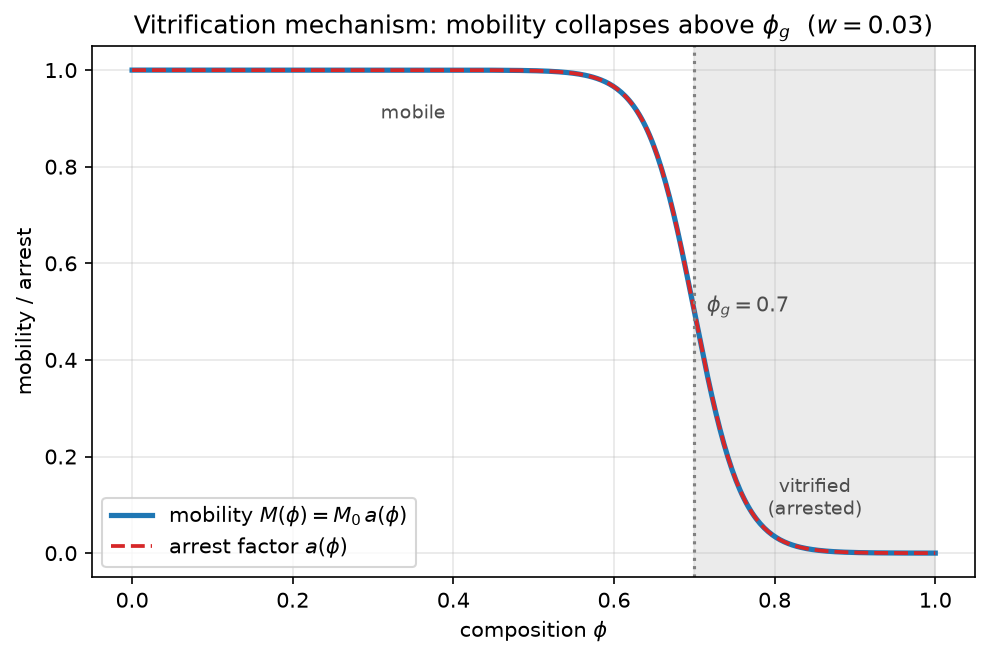
\includegraphics[width=0.72\linewidth]{figures/p11_mechanism.png}
  \caption{The added term: a composition-dependent mobility $M(\phi)=M_0a(\phi)$
  whose vitrification arrest factor $a(\phi)$ collapses the mobility above the
  glass composition $\phi_g$.}
  \label{fig:p11mech}
\end{figure}

\paragraph{Discretisation.} On a periodic grid of $N$ nodes (spacing $h$), the
Laplacian is the central second difference and the flux divergence uses an
arithmetic face-averaged mobility $M_{i+1/2}=\tfrac12(M_i+M_{i+1})$, which keeps
the analytic Jacobian clean. Time stepping is backward Euler, giving the
residual
\begin{equation}
  R(\phi) = \frac{\phi-\phi^{\,n}}{\Delta t}
          - \grad\!\cdot\!\big(M(\phi)\,\grad\mu(\phi)\big).
  \label{eq:p11res}
\end{equation}

\section{The analytic Jacobian}

The heart of a solver contribution is a correct analytic Jacobian. Writing the
discrete flux divergence as $D(\phi)$, the Jacobian of \eqref{eq:p11res} is
\begin{equation}
  J = \frac{1}{\Delta t}\,\mathbf{I} - \dd{D}{\phi},\qquad
  \dd{D}{\phi} = A_{\mathrm{mob}} + A_{\mathrm{op}}\,J_\mu,
  \label{eq:p11jac}
\end{equation}
where $J_\mu = \mathrm{diag}\,f''(\phi) - \kappa\,\mathbf{L}$ is $\dd{\mu}{\phi}$,
$A_{\mathrm{op}}$ is the flux-divergence operator with the face mobilities
frozen, and $A_{\mathrm{mob}}$ is the extra term from differentiating the face
mobilities through $M'(\phi)$. All three blocks are assembled by hand (never by
autograd) in \code{jacobian}; the derivation is written out in the module
docstring.

\paragraph{Derivative test (the gate).} The hand-derived Jacobian is checked
column-by-column against a central-difference Jacobian of the residual on a
random smooth state: the maximum absolute error is $\PelevenJacFDerr$. As an
independent cross-check, the same analytic matrix matches PyTorch autograd to
$\PelevenJacAGerr$ --- confirming the by-hand chain rule is exact, not merely
consistent with its own finite differences. The free-energy derivatives $f'$,
$f''$ are likewise checked against central differences ($\PelevenFprimeErr$,
$\PelevenFppErr$).

\section{Verification}

\paragraph{Limiting case: the Cahn--Hilliard dispersion.} With arrest off
($\phi_g\to\infty$, constant mobility) the linearised dynamics about
$\bar\phi=\tfrac12$ has the exact growth rate
$\sigma(k) = -M_0 k^2\big(f''(\bar\phi)+\kappa k^2\big)$. Measuring the
single-mode amplitude change over one backward-Euler step reproduces it: at the
fundamental mode $\sigma_{\text{measured}}=\PelevenSigMeas$ against
$\sigma_{\text{analytic}}=\PelevenSigAna$ (relative error $\PelevenDispRelErr$),
and the whole $\sigma(k)$ curve tracks the analytic one
(Fig.~\ref{fig:p11disp}).

% --- generated by gen_figures.py ---
\begin{figure}[h]\centering
  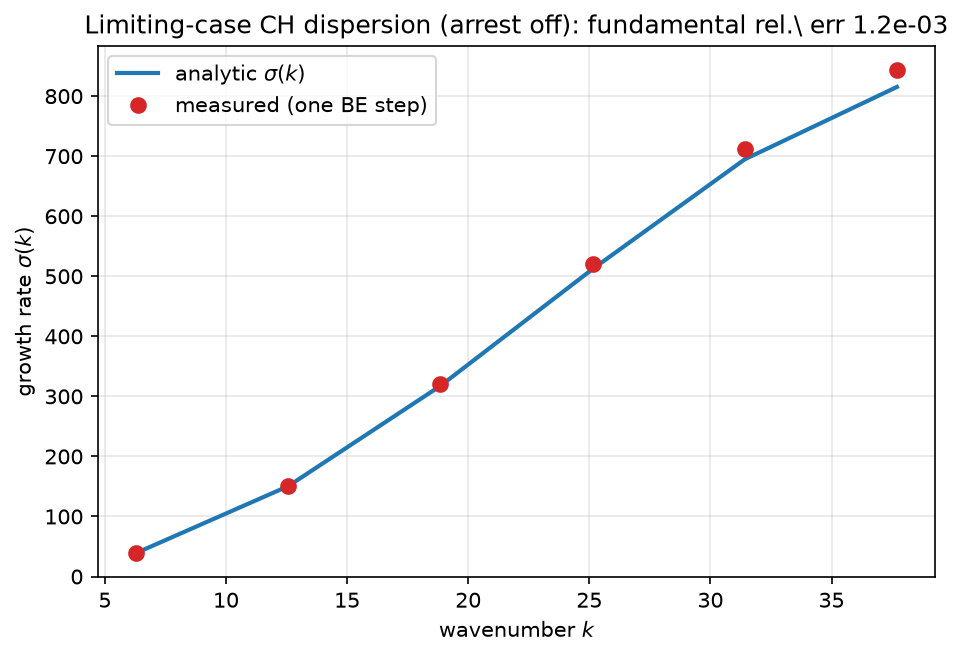
\includegraphics[width=0.62\linewidth]{figures/p11_dispersion.png}
  \caption{Limiting-case verification: with the arrest switched off the measured
  single-mode growth rate matches the analytic Cahn--Hilliard dispersion
  $\sigma(k)$.}
  \label{fig:p11disp}
\end{figure}

\paragraph{Manufactured solution and orders of accuracy.} A manufactured
solution $\phi^*(x,t)=\bar\phi + A\sin(qx)e^{-\lambda t}$ with its exact analytic
source added to the residual gives a clean spatial convergence study: the
$L_2$ error against $\phi^*$ falls from $\PelevenMMSerrCoarse$ to
$\PelevenMMSerrFine$ under mesh doubling, an observed order of $\PelevenMMSorder$
(minimum $\PelevenMMSorderMin$) --- the expected second order of the
central/face-averaged discretisation. Refining the time step instead recovers
the first-order backward-Euler rate $\PelevenTempOrder$
(Fig.~\ref{fig:p11conv}). Mass is conserved to $\PelevenMassDrift$ over the
scientific run, and Newton converges in at most $\PelevenNewtonIters$ iterations.

% --- generated by gen_figures.py ---
\begin{figure}[h]\centering
  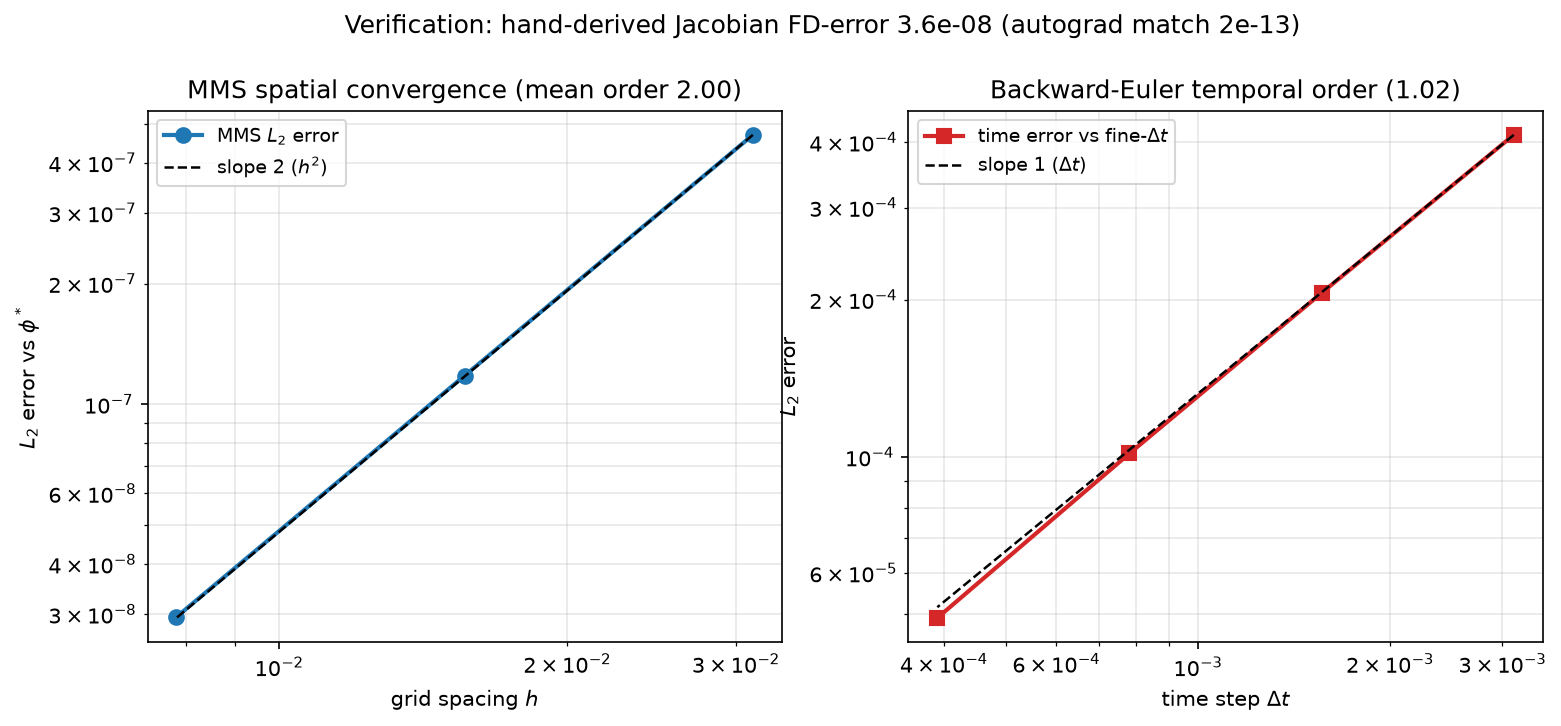
\includegraphics[width=\linewidth]{figures/p11_convergence.png}
  \caption{MMS spatial convergence (left, second order) and temporal convergence
  (right, first order for backward Euler), each against its theoretical
  reference slope.}
  \label{fig:p11conv}
\end{figure}

\section{GPU profile}

A new mechanism ships with a \emph{measured} cost. \code{profile\_gpu.py} times
one full Newton step (residual $+$ analytic-Jacobian assembly $+$ dense solve)
against grid size $N$ on both devices (Fig.~\ref{fig:p11prof}). At $N=\PelevenProfMaxN$
the step costs $\PelevenProfMs$~ms on the \PelevenProfDevice\ device at a peak of
$\PelevenProfPeakMB$~MB, a $\PelevenProfSpeedup\times$ speedup over the CPU.
Honestly, at small $N$ the CPU wins: this brick forms a \emph{dense}
$N\times N$ Jacobian and the GPU only repays its launch overhead once $N$ is
large. That is the right lesson --- profile before assuming the GPU helps, and
know that the production path (Chapter~\ref{ch:c7}) uses a sparse assembly for
exactly this reason.

% --- generated by gen_figures.py ---
\begin{figure}[h]\centering
  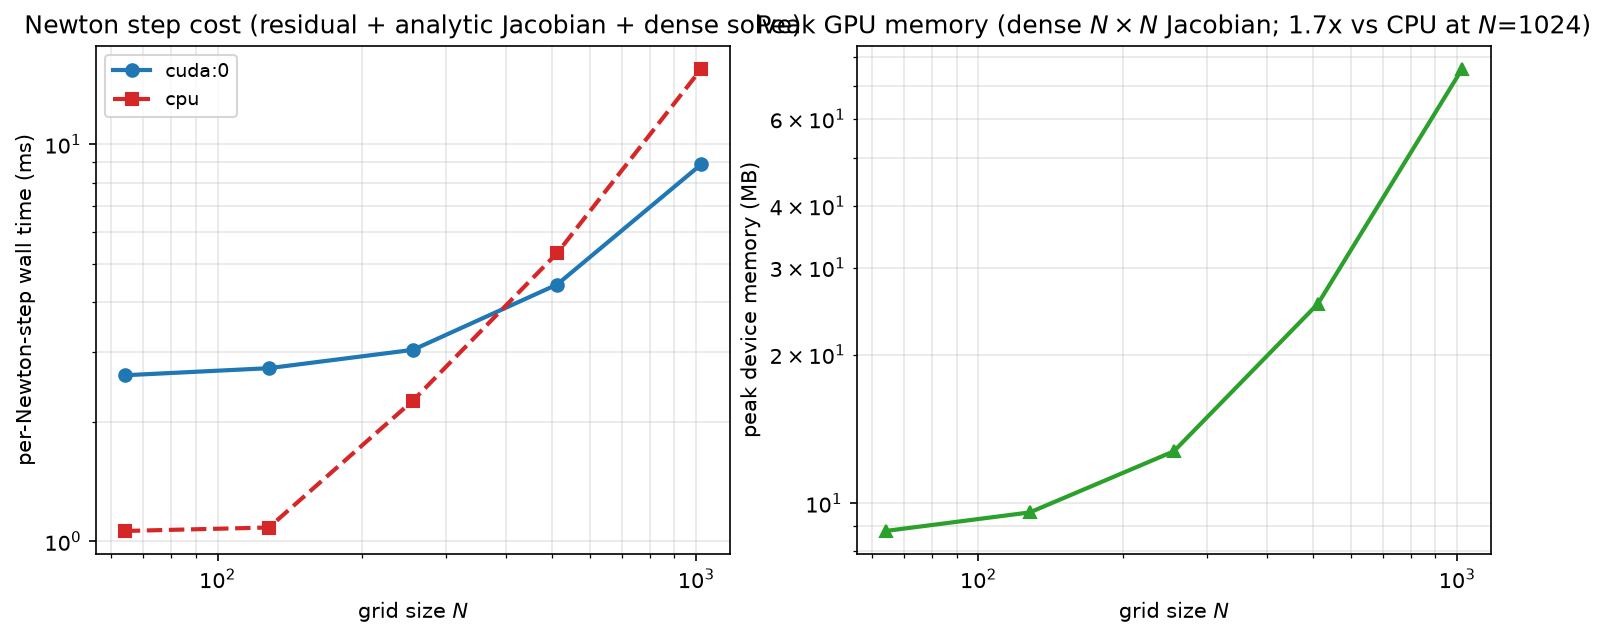
\includegraphics[width=\linewidth]{figures/p11_profile.png}
  \caption{GPU profile of the Newton step: wall time vs grid size $N$ (left,
  GPU vs CPU) and peak device memory (right). The dense $N\times N$ Jacobian
  makes the GPU worthwhile only at larger $N$.}
  \label{fig:p11prof}
\end{figure}

\section{The scientific result}

With every check green we can trust the physics. Starting from a random initial
condition at the glass composition (so the polymer-rich matrix vitrifies), a
run \emph{without} arrest coarsens --- the domain length $L(t)$ grows to
$\PelevenLfree$ --- while the vitrified run \emph{arrests}: $L(t)$ plateaus at
$\PelevenLarrest$ (a last-half growth of only $\PelevenPlateauGrowth\%$), a
factor $\PelevenArrestRatio$ finer (Fig.~\ref{fig:p11coarsen}). This is the
mechanism that stops the clock in Chapter~\ref{ch:p10}: vitrification freezes a
fine, non-equilibrium morphology instead of letting it coarsen to a coarse
equilibrium --- precisely what makes a fast-dried organic film's morphology
kinetically selectable.

% --- generated by gen_figures.py ---
\begin{figure}[h]\centering
  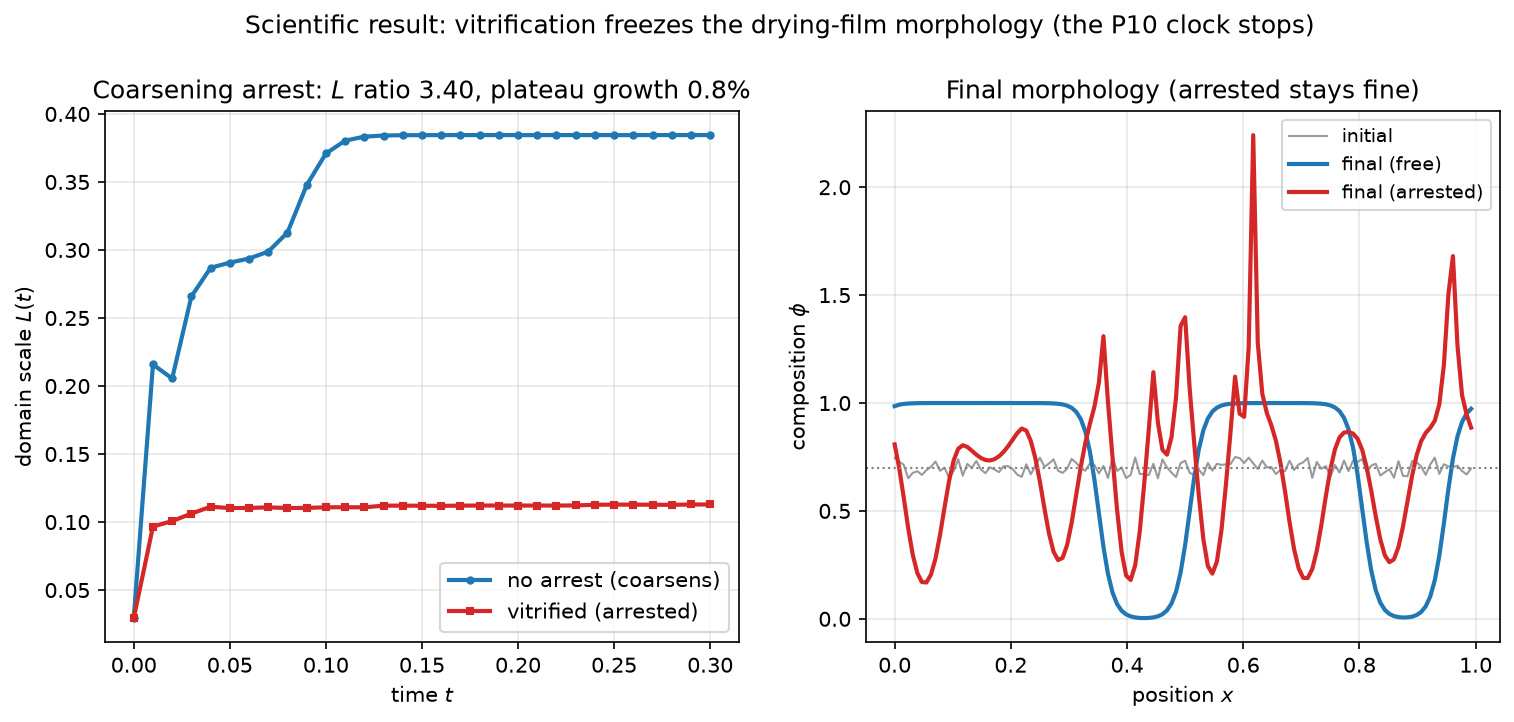
\includegraphics[width=\linewidth]{figures/p11_coarsening.png}
  \caption{Scientific result: without arrest the domains coarsen ($L$ grows);
  with the polymer-rich matrix vitrified, coarsening halts and a fine morphology
  is frozen in.}
  \label{fig:p11coarsen}
\end{figure}

\begin{runbox}
\textbf{Run it.}
\begin{lstlisting}
cd physics/11_model_extension
python -m pytest test_vitrification.py -q          # the derivative + MMS gates
python run_harness.py --config configs/p11.yaml --mode reference \
    --output outputs/p11 --overwrite               # results.json vs baseline.yaml
python profile_gpu.py --run-dir outputs/p11        # the GPU profile
python gen_figures.py --run-dir outputs/p11        # figures + numbers
\end{lstlisting}
The brick is entirely tutorial-local (\file{vitrification.py}); it does not touch
the core \file{src/} solver, so it is a template for a first contribution.
\end{runbox}

\section{The contributor checklist}

This is the workflow a real mechanism PR follows (spec C8), all exercised here:

\begin{keybox}
\textbf{From term to merged mechanism.}
\begin{itemize}[nosep]
\item derivation of the term and its continuous operator (\S1);
\item a residual and an \emph{analytic} Jacobian, assembled by hand (\S2);
\item a finite-difference derivative test --- the non-negotiable gate --- plus
  an autograd cross-check (\S2);
\item a limiting case with a known closed-form answer (the CH dispersion, \S3);
\item an MMS spatial-convergence study at the design order, and the temporal
  order (\S3);
\item a conservation check (\S3);
\item a GPU profile with an honest cost verdict (\S4);
\item a tolerance-checked scientific result (\S5); and PR-quality docs
  (\file{README.md} + this chapter).
\end{itemize}
\end{keybox}

\section{Explore on your own}

\question{Replace the sigmoid arrest with a power-law degenerate mobility
$M(\phi)=M_0\,\phi(1-\phi)$ and re-derive $M'(\phi)$. Update \code{Mmob} and
\code{Mprime}, then confirm the finite-difference Jacobian test still passes ---
the derivative test catches a wrong $M'$ immediately.}

\question{Make the arrest width $w$ smaller and re-run the coarsening study. How
sharp must the glass transition be before the arrested domain scale stops
depending on $w$? Relate this to the interface width $\sqrt{\kappa}$.}

\question{The GPU profile shows the dense solve losing to the CPU at small $N$.
Sketch what a sparse (tridiagonal-plus-mobility) assembly would change, and at
what $N$ you would expect the crossover to move. Connect to Chapter~\ref{ch:c7}.}

\question{Extend the mechanism to two dimensions (the field becomes $N\times N$).
Which of the verification steps (derivative test, MMS, dispersion) transfer
unchanged, and which need a 2-D manufactured solution?}
